

\subsection{LED controller}

The LEDs are powered by a 12V supply. As this voltage can not be supplied directly from the FPGA, a driver is needed.
Because of that, the LEDs are driven with a MOSFET driver. This transistors allow us to turn on and off the LEDs with a output signal from the FPGA using a minimum current from the integrated circuit at high frequencies.

The selected transistor for this driver has been a NTD5867NL. This n-Channel MOSFET is able to drive up to 60V and 20A with a gate-to-source threshold voltage of 2.5V, what makes it perfet to drive the LEDs with a FPGA signal.
Apart from that, these MOSFET have a drain-to-source resistance of up to 50 m$\Omega$ (which can be ignored), and can be driven up to 30MHz.

In this project the LEDs are going to be turn on and off with a frequency of up to 170kHz, so the MOSFET is fast enough for this application.

In figure \ref{fig:LED_driver_sch} the schematics for the LED driver are shown.

The selected LED colors for this project has been red, green and blue. Using the information given by the manufacturer, the resistor used to limit the current in the LEDs has been chosen. The selected resistors has been 1k$\Omega$ for the blue and green colors and 430$\Omega$ for the red one.

\begin{figure}[H]
\centering 
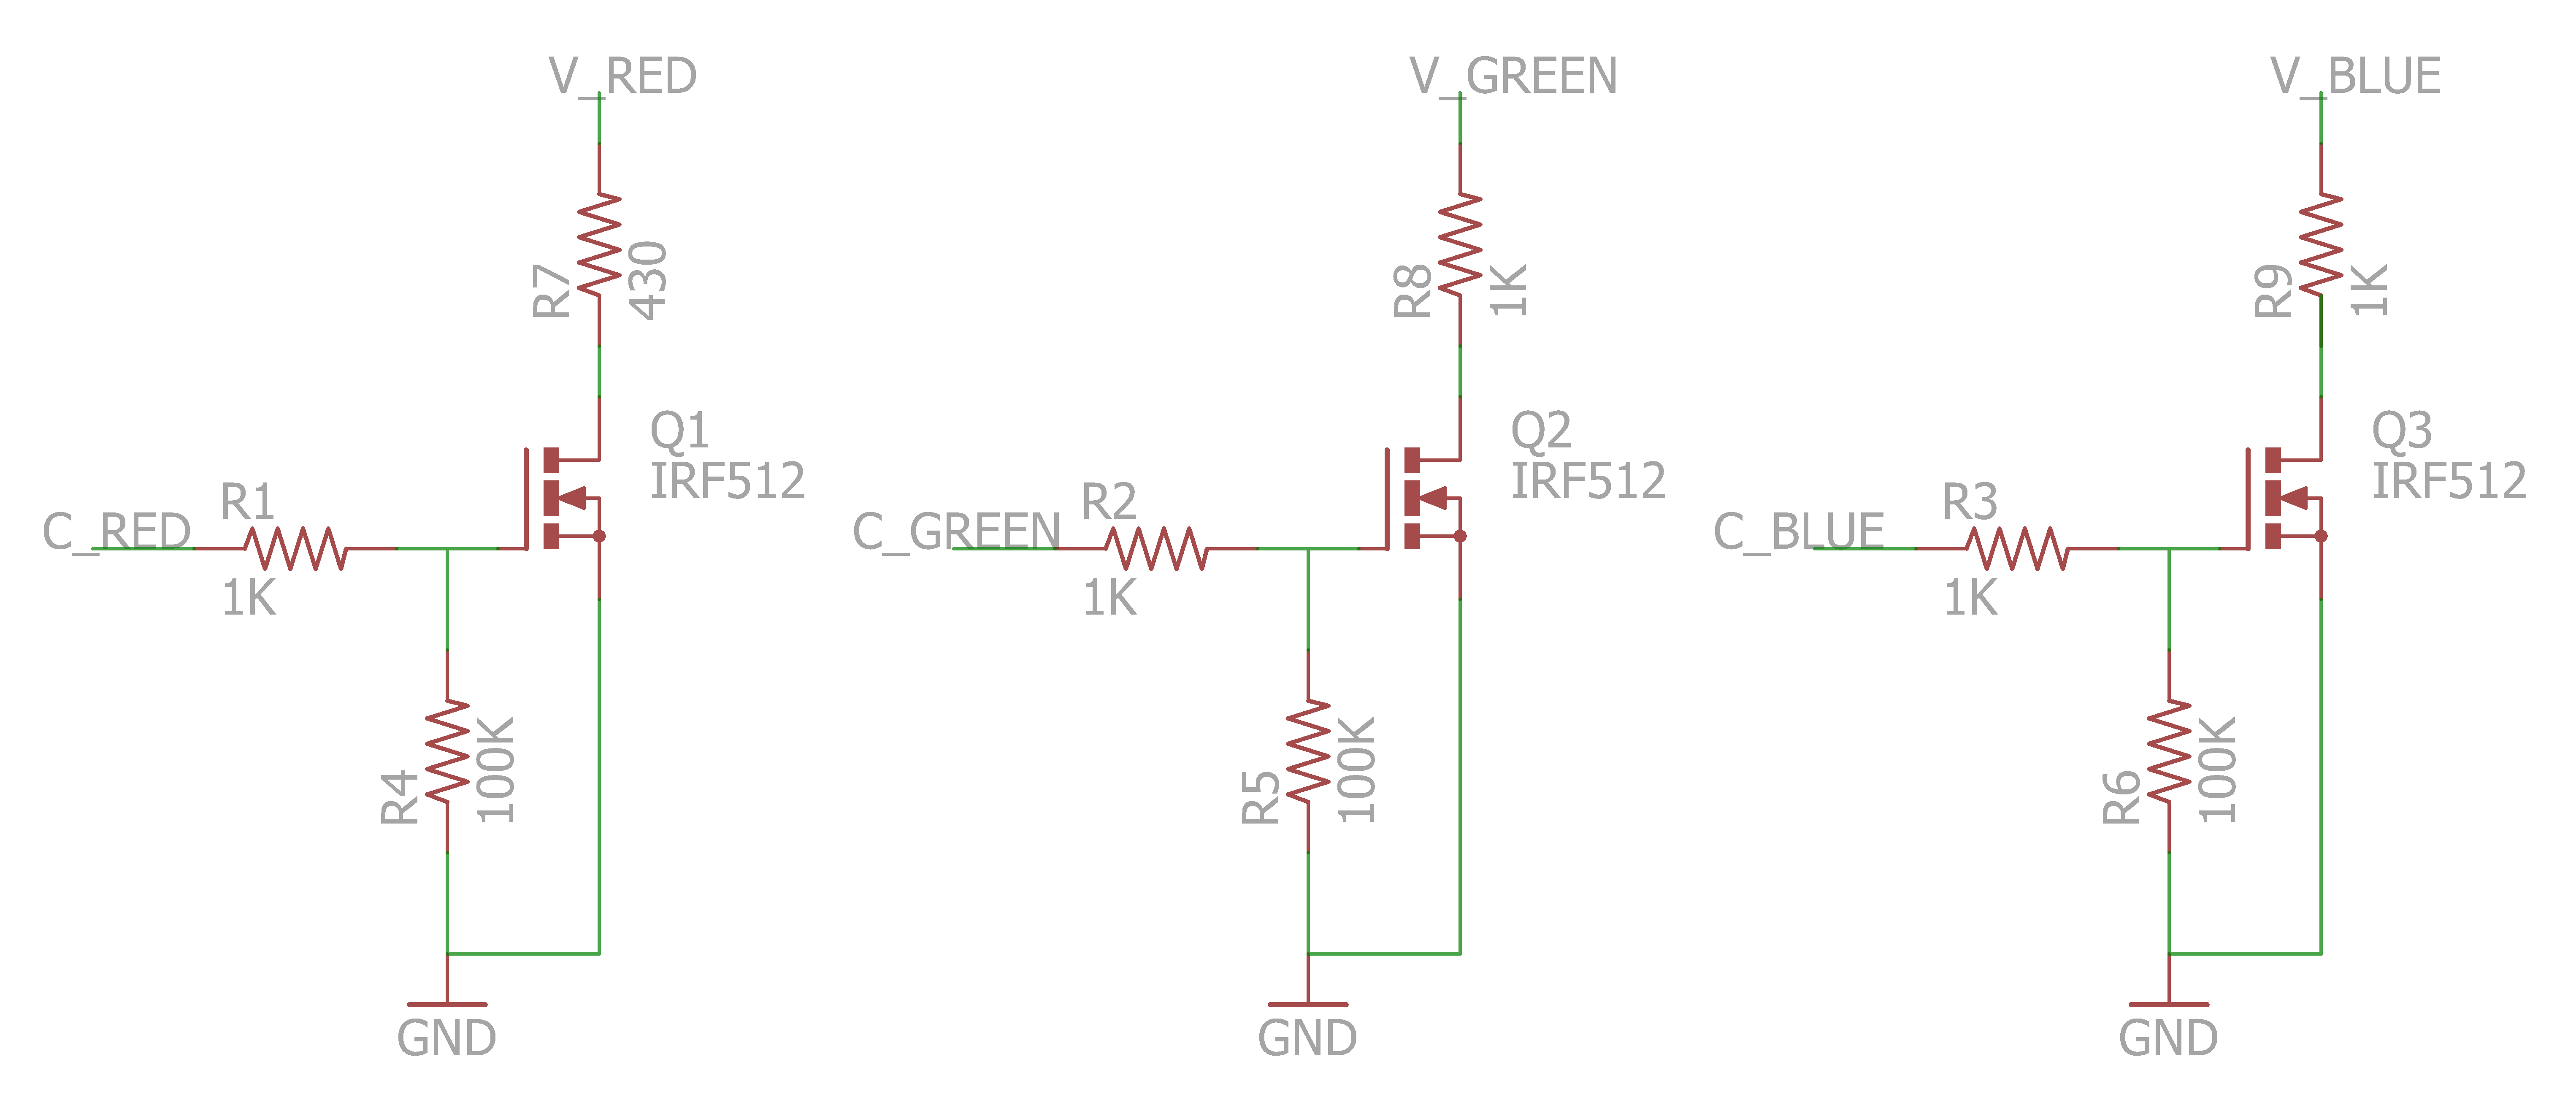
\includegraphics[width = 0.4 \textwidth]{images/leddriver_schematics}
\caption{...}
\label{fig:LED_driver_sch}
\end{figure}